\documentclass[11pt]{article}

\usepackage[margin=1in]{geometry}
\usepackage[T1]{fontenc}
\usepackage{microtype}
\usepackage{booktabs}
\usepackage{tabularx}
\usepackage{array}
\usepackage{enumitem}
\usepackage{amsmath,amssymb}
\usepackage{xcolor}
\usepackage{xurl}
\usepackage{hyperref}
\usepackage{natbib}
\usepackage{graphicx}
\usepackage{placeins}
\graphicspath{{figures/}}

\hypersetup{
  colorlinks=true,
  linkcolor=blue!70!black,
  citecolor=blue!70!black,
  urlcolor=blue!70!black
}

\newcommand{\eetwo}{\textsc{E2E-Exact}}
\newcommand{\pp}{percentage points}
\newcolumntype{Y}{>{\raggedright\arraybackslash}X}
\newcolumntype{C}[1]{>{\centering\arraybackslash}p{#1}}
\setlength{\emergencystretch}{3em}

\title{When Not to Generate:\\
       How AI Systems Quote Scripture, and What\\
       Authoritative Quotation Requires}

\author{Alex Chao\\
        \textit{Fide AI}\\
        \texttt{alex@fideai.org}}

\date{July 2026}

\begin{document}
\maketitle

\begin{abstract}
People increasingly ask AI assistants for Scripture---in sermon preparation,
teaching, and pastoral conversation. These are not ordinary information
requests: someone asking for a passage wants particular words, in a particular
translation, from a source they could have opened themselves. A reply that
blends two translations, drops a verse, or paraphrases inside quotation marks
satisfies none of that while appearing to satisfy all of it, and the person who
asked is the one least able to check. Existing evaluation does not see this
failure. A response can be factually accurate, properly cited, and semantically
faithful, and still be the wrong text.

When the words themselves are the answer, who should be responsible for them?
We route matched Scripture requests through four designs---the model quotes
from memory; the passage is placed in front of it to copy; it is given a lookup
tool; or it only names the passage and non-generative code inserts the text.
Locked in advance, the study covers 8,640 requests across six model families,
three open English editions, and twenty passages. Quoting from memory produced
the requested edition exactly 25.00\% of the time; supplying the text raised
that to 93.61\%, a lookup tool to 80.09\%, and deterministic insertion to
83.94\%. The central finding is that connecting a source did not remove failure
but moved it onto whatever the model still decided. Models called the tool in
95.00\% of cases yet asked it for the right passage in only 84.17\%.
Deterministic insertion was near-perfect once the model named the right
passage---1,813 of 1,815---and powerless when it did not. Exact quotation is
not one skill but a chain, and each link fails on its own terms. This measures
textual delivery, not whether a passage was well chosen, rightly interpreted,
or pastorally apt.
\end{abstract}

\section{Introduction}
\label{sec:introduction}

Consider three requests a person might make of an AI assistant. ``Give me
Ephesians 2:8--9 in the Berean Standard Bible for Sunday's slide.'' ``Quote the
passage where Jesus compares his being lifted up to Moses' serpent in the
wilderness.'' ``Send me Revelation 21:1--4 to read at a funeral.''
Each asks for exact words, but each puts a different decision in the system's
hands. The first names the passage and the edition, leaving only faithful
reproduction. The second names neither, so the passage must be identified
before it can be quoted. The third is long enough that truncation, not
misidentification, is the likely failure. An assistant that answers all three
the same way---by generating fluent text that carries the right
reference---fails each of them differently, and the final prose does not reveal
which failure occurred.

That opacity is the practical problem. The meaning may survive a blended or
shortened rendering; the quotation does not. And the person who asked is poorly
placed to notice, because checking the answer would require already having the
text they asked for. For requests like these, wording is not merely a vehicle
for the answer. Wording is part of the answer.

These requests are not hypothetical, and the settings are not peripheral. In a
December 2025 survey of U.S. Protestant pastors, 87\% reported using AI in
ministry, 36\% for biblical or theological research, and 24\% for writing or
editing sermons \citep{barna2026pastors}. A separate survey of 594 church
leaders found comparable adoption alongside near-absent governance: most
reported frequent use, while 73\% reported no AI policy of any kind
\citep{exponential2025aichurch}. Which English translation a person reads is
itself a durable, measurable feature of American religious life rather than an
incidental preference \citep{goff2017bible}, so substituting one edition for
another is not a cosmetic error.

The stakes are practical and specific. A congregation reads responsively from a
printed edition while a screen displays different wording. A student memorizes
a verse in one translation and is later corrected against another. A teacher
builds an argument on a clause that the quoted edition does not contain.
Someone in distress receives a passage with its final line missing. In each case
the response is fluent, carries the right reference, and is wrong in the way
that matters. Readers reasonably treat quotation marks and a verse reference as
a claim about a source of record; when that claim is unreliable and difficult
to detect, the cost falls on the reader rather than on the system.

Practitioners have noticed. The chief executive of a major digital Bible
platform has publicly estimated that leading models misquote Scripture between
15\% and 60\% of the time, and has cited that estimate as a reason not to ship
a Scripture-answering assistant \citep{gruenewald2026misquotes}. The estimate
is plausible and consequential, but no measurement protocol accompanies it: the
systems, passages, editions, and criterion for ``misquote'' are unstated, so it
can be neither checked nor acted on with confidence. Claims of that importance
deserve a specified, reproducible measurement. Providing one, for a bounded set
of English editions and conditions, is the purpose of this paper.

We use \emph{authoritative quotation} to mean delivering the requested span, in
the requested edition, from an identified source of record---a specific,
versioned text designated as authoritative for that request, rather than an
abstract notion of authority. A response may be relevant, factually close, or
theologically unobjectionable while still failing that narrower task. It may
silently substitute an edition, blend familiar formulations, omit a verse,
expand beyond the requested span, or present a paraphrase as a quotation. This
is a stricter requirement than factuality, attribution, or groundedness: a
response can be factually supported and properly cited while still failing an
exact quotation request.

Neither model scale nor retrieval resolves the problem on its own. Language
models are built to generate plausible continuations; parametric memory can
sometimes reproduce a familiar source verbatim, but it is not a
source-of-record interface. Retrieval can make authoritative text available,
and a generative layer can still alter it. A model holding a tool can bypass
the tool or request the wrong span. A deterministic renderer can preserve
source bytes exactly, but only downstream of a correct decision about source,
edition, and boundaries. Return to the serpent request above and the point
sharpens: a model answering from memory may blend familiar translations; a
model given the source may shorten it; a tool-enabled model may retrieve the
neighboring verse; and a deterministic renderer may reproduce the source
perfectly after the model selected the wrong range. The four designs fail at
four different places, and every one of them produces credible prose.
Authoritative quotation is a property of the whole source-delivery chain, not a
model knowledge property.

We therefore hold the user's request fixed and vary which component owns the
words. Matched requests were routed through four architectures: generation from
model memory, reproduction of source text supplied in context, retrieval
through an authorized \texttt{get\_passage} tool, and model selection of a
structured reference followed by deterministic rendering. The prospectively
specified and internally hash-locked design contains 8,640 observations across
six model families, three open English editions, twenty passages, two prompt
forms, and three repetitions. This is a matched crossed comparison rather than
a benchmark or leaderboard, and the primary endpoint is deliberately
demanding: the user-visible output must equal the requested text exactly, with
condition-specific evidence that the declared architecture was actually
followed. Scripture makes this comparison unusually tractable---verse
references supply a conventional addressing scheme, multiple English
translations make edition identity observable rather than assumed, span length
can be varied systematically, and indirect prompts force semantic
identification before rendering.

The results are stark and, we think, more interesting than a ranking. Native
generation from model memory met the strict endpoint in 25.00\% of
observations, against 93.61\% for source-supplied quotation, 80.09\% for
tool-mediated retrieval, and 83.94\% for deterministic rendering. Because the
endpoint requires the \emph{requested} edition, much of the native gap is
edition substitution rather than general unfamiliarity: native exactness ranged
from 41.53\% for the Berean Standard Bible to 5.00\% for the Literal Standard
Version. The central finding is what
happened after a source was connected. Failure did not disappear; it migrated
toward whichever decision the architecture still left to the model. A source
tool was invoked in 95.00\% of tool observations but used for the requested
lookup in only 84.17\%. Deterministic rendering was exact in 1,813 of 1,815
cases once the model had selected the correct reference---but the model
selected correctly in only 84.03\% of observations, and no renderer can repair
a wrong selection. Each architecture made one stage reliable and left another
exposed.

What transfers from this is the structure, not the numbers. The same shape
appears wherever a source of record exists: a dosing instruction, a statutory
subsection, an indemnity clause, and a safety standard each have an edition, a
boundary, and wording that a paraphrase does not preserve, and each can fail at
selection, access, rendering, or final output. The decomposition and evaluation
design developed here apply to those settings directly. The measured rates do
not---every number in this paper is about English Bible quotation, and another
domain needs its own sources, scenarios, and expertise. Many faith traditions
likewise designate specific textual forms as authoritative and treat exact
wording as consequential, but the unit of authority differs---a source-language
consonantal text, a recited form, a received translation, a commentary
tradition---and those differences would change the study design, not only the
results. We report on English Christian Bible editions and make no claim about
any other tradition's texts. Textual fidelity is also not theological fidelity:
the study evaluates whether a system delivered the requested source faithfully,
not whether the passage was well chosen, rightly interpreted, or pastorally
appropriate.

\paragraph{Contributions.}
The paper makes three contributions. First, it gives a rigorous empirical
account of Scripture quotation across twenty passages, three open English
editions, six model families, and four system architectures. Second, it defines
a \emph{source-delivery chain} that separates source selection, authorized
access, exact rendering, and final-output integrity, and shows that quotation
failures are only interpretable when attributed to a stage. Third, it releases
an open evaluation methodology, deidentified derived scores, and reproducible
analyses while keeping private execution code, raw model traces, and
rights-constrained text outside the public artifact. The study answers a public
call for research on sacred-text fidelity \citep{fid056call}, and the
repository records which parts of that call remain open. Three questions organize
the study: how architecture-adherent exactness differs across the four
architectures; at which stage failures occur; and how prompt form, passage
length, edition, model family, and repeated sampling interact with those
failures.

\section{Authoritative Quotation as a Systems Problem}
\label{sec:systems-problem}

\subsection{Quotation succeeds only when the whole chain succeeds}

A successful quotation needs four things to go right. The system must identify
what text the user means, obtain it through the declared path, preserve its
wording, and deliver that wording intact. Failure at any one stage defeats the
quotation request even if every other stage succeeds.

Formally, let a request specify, explicitly or implicitly, a source work $W$,
an edition $E$, and a span $B$. Let $T(W,E,B)$ be the authoritative text
returned by the source of record. We separate four system properties:

\begin{itemize}[leftmargin=*,topsep=4pt,itemsep=2pt]
  \item $S$: the intended work, edition, and span are selected correctly;
  \item $A$: the declared source-access method is followed and the requested
        source is available;
  \item $R$: the selected source text is rendered without alteration; and
  \item $I$: the user-visible final output preserves that rendering without
        truncation, leakage, or extraneous text.
\end{itemize}

The strict endpoint is conjunctive:

\begin{equation}
  \eetwo = S \land A \land R \land I.
  \label{eq:e2e}
\end{equation}

The operational evidence for each term depends on architecture. In native
generation there is no external access event to verify; exact final output is
the decisive behavior. In a tool condition, access requires an observed call
for the requested span rather than merely the presence of a tool definition.
In a deterministic condition, exact rendering is meaningful only after a
parseable, correct reference has reached the renderer.

This decomposition prevents a common category error. A renderer may provide a
strong guarantee about $R$ while the overall system still fails because $S$ is
false. Conversely, a model may identify the correct passage while a generative
surface layer changes the words. An aggregate score is useful, but stage-level
evidence is required to explain it.

\subsection{Why factuality and citation are not enough}

A quotation can be factually supported yet textually wrong. A citation can
point to the correct document while the quoted span omits a limiting clause.
A semantic similarity score can treat two Bible translations as nearly
equivalent even when the user requested one exact edition. Authoritative
quotation is therefore stricter than factuality, attribution, or general
groundedness.

The requirement is also narrower. The evaluation does not ask whether the source
itself is true, wise, clinically appropriate, legally controlling, or
theologically interpreted correctly. It asks whether a system delivered the
requested source faithfully under its declared architecture.

\subsection{Scripture as the study domain}
\label{sec:scripture-domain}

Scripture warrants study because AI systems increasingly mediate access to
texts that Christian communities receive, interpret, and transmit as
authoritative, and because the domain makes the quotation problem measurable. A
reference such as ``John 3:16'' identifies a conventional verse span but not
one English wording, so edition identity is observable rather than assumed. An
event-style request adds a prior selection problem: the system must identify
the intended span before it can quote it. Few domains combine a stable
addressing convention, multiple simultaneously authoritative editions, and a
community that treats exact wording as consequential.

Working here requires textual and theological restraint. The English editions
studied sit within a complex manuscript and translation history in both the
Hebrew Bible and New Testament \citep{tov2012textual,metzger2005text}, and
translation requires linguistic and interpretive decisions
\citep{nida1969theory}. The three editions differ not only in translation
philosophy but in underlying text-critical basis, so ``edition'' is partly a
claim about source-language witnesses rather than purely a matter of English
wording. The twenty targets were not selected to probe variant units, and a
study designed around textual variants would be a distinct and worthwhile
contribution. Exact reproduction of a selected English edition is therefore not
fidelity to the Hebrew, Aramaic, or Greek source texts, and no result here
establishes that one English translation is doctrinally or linguistically
superior. The twenty targets all fall within books shared by the major
Christian canons; the study does not adjudicate canonical boundaries, and the
three editions carry the Protestant canon.

For churches and Christian institutions, the practical implication is
correspondingly bounded. A system that quotes the requested edition exactly
removes one avoidable textual failure. It does not replace biblical
scholarship, ecclesial authority, pastoral judgment, or attention to literary
and canonical context. Exact quotation is a prerequisite for some forms of
responsible use, not a complete account of responsible use.

\section{Related Work}
\label{sec:related-work}

Retrieval-augmented generation combines parametric sequence models with
retrieved evidence \citep{lewis2020retrieval}. Later work examines when
parametric memory is insufficient and non-parametric memory should be preferred
\citep{mallen2023when}, while RAGAs evaluates retrieval and generation quality
within retrieval-augmented systems \citep{es2024ragas}. Tool-use research asks
whether models can decide when and how to invoke external APIs
\citep{schick2023toolformer,ross2025when2call}, and grammar-constrained
decoding offers one way to enforce structured interfaces
\citep{geng2023grammar}. Authoritative quotation joins these concerns: the
system must obtain a declared span, demonstrate that the intended access path
was used, and preserve the result.

Fine-grained factuality work decomposes long-form generation into checkable
claims \citep{min2023factscore}, while citation-oriented systems evaluate
whether generated claims are accompanied by supporting sources
\citep{gao2023alce}. Surveys document broad forms of unsupported and
unfaithful neural generation \citep{ji2023survey,huang2023survey}. Our task is
stricter in wording and narrower in scope: a response can be factually
supported and properly cited while still failing an exact quotation request.

CopyBench measures literal and non-literal reproduction of copyrighted fiction books
\citep{chen2024copybench}, while Quote-Tuning increases verifiability by
aligning models to quote verbatim strings found in trusted pretraining corpora
\citep{zhang2025verifiable}. The present study differs in object and
architecture: the requested edition and span are specified as source-of-record
requirements, and authorized retrieval or deterministic rendering can replace
parametric reproduction. These works are complementary and bound the novelty
claim; this paper does not claim to introduce verbatim-copy measurement or
quoting as a general research problem. Training-data extraction and
memorization studies likewise show that models can reproduce memorized content
under some conditions
\citep{carlini2021extracting,carlini2023quantifying}. Memorization does not
make parametric recall a stable or authorized source interface. Copyright
policy work, including the United States Copyright Office's generative-AI
training report, provides further context for making source access and
redistribution assumptions explicit \citep{usco2025ai}.

Holistic and behavioral evaluation emphasizes scenario coverage, multiple
metrics, and tests of specific capabilities rather than one undifferentiated
score \citep{liang2022helm,ribeiro2020checklist}. We adopt that orientation
without turning the study into a ranking exercise. The contribution is the
source-delivery chain: a matched evaluation of which component selected,
obtained, rendered, and preserved the requested source.

\section{Study Design}
\label{sec:study-design}

The experiment holds the request panel fixed and changes the route by which a
quotation reaches the user. This makes architecture, rather than passage choice
or model mix, the primary comparison.

\subsection{Prospective specification and execution boundary}

The primary study was prospectively specified and internally hash-locked before
confirmatory execution began. This was not a public registry deposit. The lock
fixed the target pack, source registry, prompt families, model routes,
conditions, repetitions, scoring rules, denominator policy, and bootstrap
procedure. Integration and calibration runs were excluded from confirmatory
estimates. Post-lock administrative changes removed administrative
stopping ceilings and divided execution into durable blocks; they did not
change a prompt, source, model, observation, score, or analysis.

The public replication package records the lock time, input digests, shared
implementation revision, and post-lock deviations. It also releases the exact
executed system and caller templates, target substitutions, functional tool
schema, and sampling/turn policy. Authoritative passage text is omitted from
the prompt artifact, but its release-safe digest is retained where applicable.

The primary phase contained:

\begin{equation}
20\ \text{targets} \times
2\ \text{prompt families} \times
4\ \text{conditions} \times
3\ \text{editions} \times
6\ \text{model routes} \times
3\ \text{epochs}
= 8{,}640.
\end{equation}

The unit of analysis is one target--prompt--condition--edition--model--epoch
observation. Conditions are paired within all other factors.

\subsection{Passage targets}

The target set is a stratified purposive panel, not a probability sample of
the Bible or of user requests. It contains five targets in each of four strata:

\begin{enumerate}[leftmargin=*,topsep=4pt,itemsep=2pt]
  \item explicit single verses;
  \item explicit short multi-verse passages;
  \item longer passages intended to expose truncation, span, or guardrail
        behavior; and
  \item event-style or semantic reference requests.
\end{enumerate}

Targets include narrative, poetry, wisdom, prophetic, Gospel, and epistolary
material. Two known intertextual or adjacent-passage relationships were
annotated rather than treated as fully independent evidence: the Shema and
great-commandment pair, and adjacent passages in John 3.

Each target had an explicit-reference prompt and an edition-neutral contextual
description. The contextual descriptions did not name the book, chapter, or
verse and were designed to avoid distinctive wording from any tested edition.
An initial review identified six descriptions requiring revision. Those six
underwent a structurally blinded focused reapproval and produced six exact
reference identifications. The original twenty-item review was not fully
blinded, so only the focused six-item result is described as blinded evidence.

\subsection{Source editions}

The full four-condition comparison used three open English editions:

\begin{itemize}[leftmargin=*,topsep=4pt,itemsep=2pt]
  \item Berean Standard Bible (BSB), a modern public-domain edition
        \citep{berean2023license};
  \item World English Bible Updated (WEBU), a public-domain translation
        \citep{weblicense}; and
  \item Literal Standard Version (LSV, 2020), released under CC BY-SA
        \citep{lsvlicense}.
\end{itemize}

These editions differ in translation philosophy and in underlying
text-critical basis, so a requested edition specifies more than a style of
English.

A source of record is a versioned artifact, so edition identity is disclosed
rather than left to the edition name. The public package includes a
release-safe source-edition record giving, for each edition, the provider and
provider-side source identifier, the edition designation, the rights basis, and
a normalized-text SHA-256 digest for each of the twenty targets. Ground truth
was verified at \texttt{2026-07-26T20:38:10Z} by two uncached retrievals
through the pinned shared runtime with matching digests; this establishes
retrieval stability, not independence of the upstream provider. The same stored
text then served as ground truth for every observation. Because the digests are
computed over whitespace-collapsed UTF-8 text, a replicator can hash their own
copy of a passage and confirm they hold the same edition text without either
party transmitting it. The record is derived from the source registry fixed by
the prospective lock and carries that artifact's digest, so the disclosure can
be checked against a commitment made before confirmatory execution.

Authoritative source text was retained privately for scoring. The public result
package contains aggregate metrics and no LSV passage text. Four restricted
editions were present in the locked registry but excluded from the primary
phase pending source and source-to-model authorization; they are listed in the
source-edition record with that status.

\subsection{Model routes and sampling}

The primary panel used one route from each of six model families:
GPT-5.6 Sol, Claude Sonnet 5, Gemini 3.5 Flash, DeepSeek V4 Pro, Kimi K3, and
GLM-5.2. These labels identify the endpoints evaluated on July 26--27, 2026;
they are not claims about later versions or general vendor performance.

Requests used OpenRouter-compatible routing with one upstream provider pinned,
fallbacks disabled, required parameter support, and data-collecting routes
denied. Provider-default sampling was used with temperature omitted. Every
cell was observed in three epochs. Semantic retries were zero. Bounded
transport retries were allowed, and terminal provider errors remained
non-deliveries in the primary denominator.

\subsection{Architecture conditions}

The four conditions give the model progressively different responsibilities.
In the first, the model must supply the words itself. In the second, the words
are already present and the model must preserve them. In the third, the model
must obtain the words through a tool and then return them. In the fourth, the
model selects only the reference; a deterministic layer owns the words. The
caller asks the same question in every matched cell, so the comparison changes
the delivery path rather than the user's request
(Figure~\ref{fig:delivery-paths}).

\begin{figure}[t]
\centering
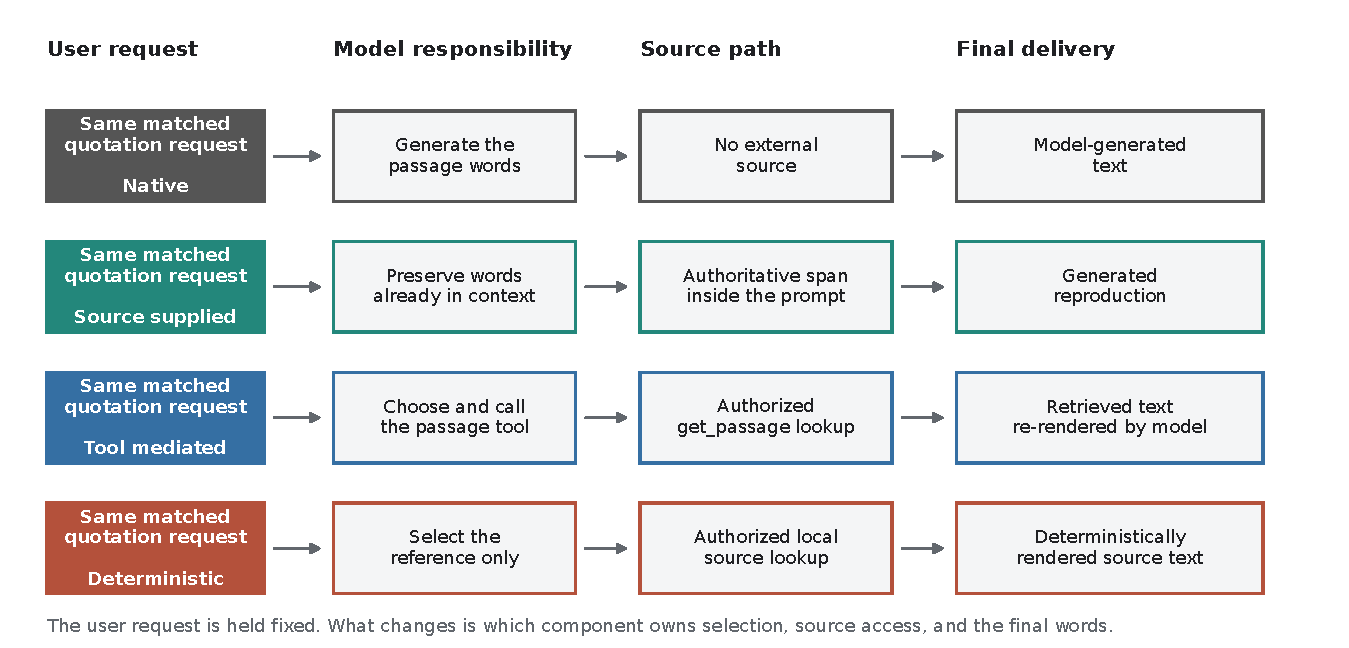
\includegraphics[width=\textwidth]{fig1_delivery_paths.pdf}
\caption{The four evaluated paths through the source-delivery chain. The
caller request is matched across conditions; what changes is which component
owns the source words and the decisions that precede them.}
\label{fig:delivery-paths}
\end{figure}

\paragraph{Native parametric quotation.}
The model received no source text and no tool. This condition represents the
common behavior of asking a general assistant to quote from memory.

\paragraph{Source-supplied quotation.}
The authoritative span was placed in the model context and the model was asked
to return it unchanged. This approximates a simple retrieval or source-injection
architecture while isolating whether the generative layer preserves available
text.

\paragraph{Tool-mediated retrieval.}
The model received an authorized \texttt{get\_passage} tool and was instructed
to use it. The trace recorded whether the tool was invoked and whether it
retrieved the requested span. Emitting text that resembled a tool call without
an executable call did not count as tool use.

\paragraph{Structured selection and deterministic rendering.}
The model was instructed to return exactly one placeholder of the form
\texttt{<quote>\{\{QUOTE:<reference>\}\}</quote>}. A local deterministic
layer parsed the reference, fetched the selected edition and span, and replaced
the placeholder. The primary score used the strict executed grammar. A
prospectively specified analysis-only tolerant parser separately assessed whether one
unambiguous expected reference could be recovered from malformed formatting;
it never changed the observed output or primary score.

\subsection{Outcomes and estimands}
\label{sec:analysis}

\paragraph{Primary and common outcomes.}

The locked primary endpoint, \eetwo, required strict final-output equality and
all condition-specific selection, lookup, replacement, and method-adherence
checks. We call it \emph{architecture-adherent exactness} throughout: the
gates differ by condition because the declared architectures differ. The
common cross-condition text outcome is final-output exactness, which asks only
whether the complete user-visible output equals the requested text. Both are
reported so that a process failure is not mistaken for a textual mismatch, or
vice versa. No weighted composite score was used. Terminal errors counted as
failures in the intention-to-observe denominator.

We also report:

\begin{itemize}[leftmargin=*,topsep=4pt,itemsep=2pt]
  \item exact and declared-normalized text match;
  \item answer presence and span coverage;
  \item strict and tolerant reference selection;
  \item tool invocation, requested lookup, and bypass;
  \item placeholder parsing and deterministic replacement; and
  \item final-output exactness and extraneous text.
\end{itemize}

Normalization covered limited surface variation and was never used to erase a
translation or edition difference. The strict endpoint remained byte-sensitive
to the protocol's expected final text after declared wrapper handling.

\paragraph{Estimands and uncertainty.}

Condition rates use all 2,160 scheduled observations per condition and are
accompanied by raw counts. The prospectively specified primary contrast is the paired risk
difference between deterministic rendering and native generation. We also
report paired source-supplied and tool-mediated contrasts. Paired intervals
come from a 10,000-resample target-cluster bootstrap with seed 5601. Clustering
by target acknowledges repeated observations of the same passage while
preserving the crossed cells inside each resample.

Model, prompt, edition, and passage-stratum analyses are descriptive
interactions. The study was not designed to rank vendors, estimate population
prevalence across Scripture, or infer training-set membership. Model routes
and editions are a fixed evaluation panel; the bootstrap does not support
generalization to untested routes or editions.

We additionally report target-level rate distributions and a post-hoc linear
probability sensitivity model with condition, route, edition, prompt-family,
passage-stratum, and epoch fixed effects and target-cluster-robust standard
errors using a $t_{19}$ reference distribution. This model was not part of the
prospective lock and is used only to test whether the primary fixed-panel
conclusions depend on the unadjusted presentation. It does not convert the
purposive target panel into a probability sample.

\section{Results}
\label{sec:results}

Three findings organize the results. First, every source-connected condition
delivered exact text substantially more often than generation from model
memory. Second, connecting a source did not remove failure; it moved failure
to a different stage of the source-delivery chain. Third, passage length and the need to
infer a reference exposed weaknesses that pooled condition rates alone would
miss. We begin with execution integrity and the primary comparison, then trace
those failures through the chain.

\subsection{The scheduled design was retained despite provider errors}

All 48 route--method--prompt-family blocks completed, yielding all 8,640
scheduled observations and unique trial and execution-request identities.
Thirty-three observations ended in terminal provider errors: 23 on the
DeepSeek route and 10 on the Kimi route. Thirty-two errors occurred in native
generation and one in tool-mediated retrieval. No semantic replacement sample
was run.

Response-level provider and response-ID metadata were present for 8,594
observations. The 46 gaps were confined to DeepSeek or Kimi native-generation
observations; 32 were terminal errors and 14 completed. The one remaining
terminal error occurred in tool-mediated retrieval and retained its provider
metadata. Requested routes still
had one upstream pinned and fallbacks disabled. We retain this as disclosed
provenance missingness rather than excluding the observations.

\subsection{Source-connected systems quoted far more exactly than generation from memory}

\begin{figure}[t]
\centering
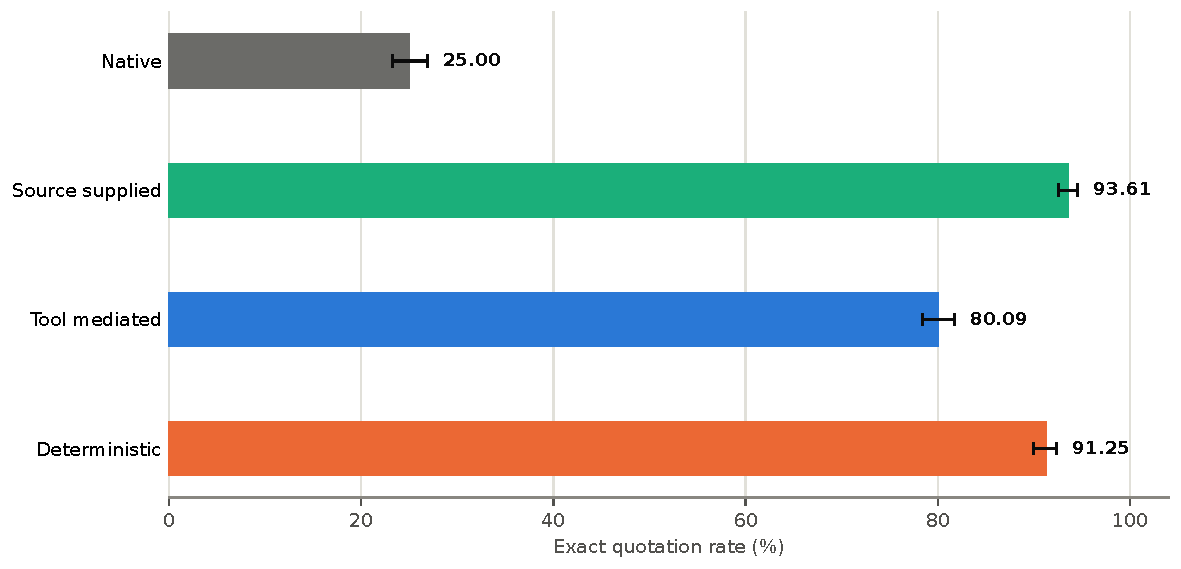
\includegraphics[width=0.88\textwidth]{fig2_condition_outcomes.pdf}
\caption{Common final-text exactness and architecture-adherent
exactness by condition. The measures differ only for tool-mediated retrieval,
where some exact final answers did not satisfy the declared tool-use gates.}
\label{fig:condition-outcomes}
\end{figure}

\begin{table}[t]
\centering
\small
\begin{tabular}{lrrrr}
\toprule
Condition & Final exact & \eetwo{} exact & $N$ & \eetwo{} rate \\
\midrule
Native parametric quotation & 540 & 540 & 2,160 & 25.00\% \\
Source-supplied quotation & 2,022 & 2,022 & 2,160 & 93.61\% \\
Tool-mediated retrieval & 1,778 & 1,730 & 2,160 & 80.09\% \\
Deterministic rendering & 1,813 & 1,813 & 2,160 & 83.94\% \\
\bottomrule
\end{tabular}
\caption{Common final-text exactness and architecture-adherent
exactness. All scheduled observations, including terminal
provider errors, remain in the denominator.}
\label{tab:primary}
\end{table}

Native parametric quotation produced an exact final quotation in one quarter of
observations (Figure~\ref{fig:condition-outcomes};
Table~\ref{tab:primary}); in other words, three out of four
requests failed the strict endpoint when the model had to supply the passage
from memory. Every source-connected intervention substantially improved on
that baseline. Source-supplied quotation had the highest pooled rate,
followed by deterministic rendering and tool-mediated retrieval. That ordering
is useful descriptively, but it does not yet explain what each architecture
made reliable.

\begin{table}[t]
\centering
\small
\begin{tabular}{lrr}
\toprule
Treatment vs.\ native & Paired risk difference & Cluster bootstrap 95\% interval \\
\midrule
Source supplied & +68.61 \pp & [+61.71, +75.60] \\
Tool mediated & +55.09 \pp & [+46.48, +63.47] \\
Deterministic rendering & +58.94 \pp & [+51.16, +66.67] \\
\bottomrule
\end{tabular}
\caption{Paired effects on architecture-adherent exactness. Complete pairs:
2,160 for each contrast.}
\label{tab:effects}
\end{table}

The prospectively specified deterministic-versus-native risk difference was
+58.94 \pp{}
(Table~\ref{tab:effects}). The source-supplied contrast was larger at +68.61
\pp{}, and the tool-mediated contrast was +55.09 \pp{}. The intervals describe
variation across the twenty target clusters, not a probability sample of all
possible Bible passages or user requests.

\begin{table}[t]
\centering
\small
\begin{tabular}{lrrrr}
\toprule
Condition & Target median & IQR & Minimum & Maximum \\
\midrule
Native parametric & 18.98\% & [10.65, 39.58] & 0.00\% & 56.48\% \\
Source supplied & 98.61\% & [92.82, 100.00] & 55.56\% & 100.00\% \\
Tool mediated & 88.43\% & [72.45, 94.44] & 34.26\% & 96.30\% \\
Deterministic rendering & 89.35\% & [83.33, 92.59] & 46.30\% & 96.30\% \\
\bottomrule
\end{tabular}
\caption{Distribution of architecture-adherent exactness across the twenty
targets. Each target rate pools the balanced route, edition, prompt, and epoch
panel ($N=108$ per condition and target).}
\label{tab:target-distribution}
\end{table}

The target distributions show that the pooled effects were not driven by one
or two passages (Table~\ref{tab:target-distribution}), but they also expose
substantial target heterogeneity. In the post-hoc cluster-robust sensitivity
model, adjusted risk differences were +68.61 \pp{} for source supplied
($t_{19}$ interval [+60.83, +76.39]), +55.09 \pp{} for tool mediated
([+45.68, +64.50]), and +58.94 \pp{} for deterministic rendering
([+50.36, +67.51]). These estimates are nearly identical to the paired
fixed-panel contrasts and are interpreted as sensitivity results, not new
confirmatory claims.

\subsection{Each architecture left a different model decision exposed}

\begin{table}[t]
\centering
\small
\begin{tabular}{lrrrrr}
\toprule
Condition & Answered & Exact text & Method adherence & Final exact & \eetwo \\
\midrule
Native & 98.29\% & 25.14\% & -- & 25.00\% & 25.00\% \\
Source supplied & 100.00\% & 93.66\% & 100.00\% & 93.61\% & 93.61\% \\
Tool mediated & 99.81\% & 82.31\% & 84.17\% & 82.31\% & 80.09\% \\
Deterministic rendering & 100.00\% & 83.98\% & 92.55\% & 83.94\% & 83.94\% \\
\bottomrule
\end{tabular}
\caption{Selected component rates. ``Method adherence'' is
condition-specific and should not be compared as a general model capability.}
\label{tab:components}
\end{table}

The aggregate rates become more informative when read as a sequence of gates
(Table~\ref{tab:components}). Source-supplied quotation removed the first two
gates: the model did not have to identify or retrieve the passage because the
authoritative span was already in context. Even so, 138 final outputs were
inexact. Making authoritative text available therefore approached, but did
not create, deterministic copying.

The tool condition reintroduced source access as a model decision. A tool invocation was
observed in 2,052 of 2,160 observations (95.00\%), but the requested retrieval
was used in only 1,818 (84.17\%). The remaining trace-level failures included
107 bypasses and 234 calls for a span other than the requested span, plus one
terminal error. Among observations satisfying tool method adherence, 1,730 of
1,818 (95.16\%) achieved architecture-adherent exactness. The tool itself was not
the guarantee; correct use of the tool was.

The deterministic condition moved responsibility again. Strict reference
selection was correct in 1,815 of 2,160 observations (84.03\%). Among those
correct selections, 1,813 produced an exact final quotation (99.89\%). Once the
correct reference crossed the interface, the renderer behaved almost
deterministically. The dominant uncertainty was upstream: whether the model
selected the right passage.

Formatting and selection were related but not identical. The outer placeholder
was recognized in 2,159 observations, while 161 observations carried a
syntax-related failure tag, usually because the model added an edition label to
the reference payload. The analysis-only tolerant parser identified the
expected reference in 1,954 observations (90.46\%), including 158 of those 161
syntax-tagged cases. This does not change the strict 83.94\% primary result.
It shows that interface conformance and semantic reference selection are
different questions.

\subsection{Contextual requests mainly challenged reference identification}

\begin{table}[t]
\centering
\small
\begin{tabular}{lrr}
\toprule
Condition & Explicit reference & Contextual description \\
\midrule
Native & 27.41\% & 22.59\% \\
Source supplied & 93.52\% & 93.70\% \\
Tool mediated & 90.19\% & 70.00\% \\
Deterministic rendering & 85.56\% & 82.31\% \\
\bottomrule
\end{tabular}
\caption{Architecture-adherent exactness by caller prompt family ($N=1{,}080$
per cell).}
\label{tab:prompt}
\end{table}

Contextual descriptions had little pooled effect on source-supplied
reproduction, where the authoritative span was already present. Their largest
effect appeared in tool-mediated retrieval: exactness fell by 20.19 \pp{}
relative to explicit references. Deterministic rendering fell by 3.25 \pp{},
consistent with the model having to identify a span before the renderer could
act.

\subsection{Long passages remained difficult even with source access}

\begin{table}[t]
\centering
\small
\begin{tabular}{lrrr}
\toprule
Condition & BSB & WEBU & LSV \\
\midrule
Native & 41.53\% & 28.47\% & 5.00\% \\
Source supplied & 94.44\% & 93.75\% & 92.64\% \\
Tool mediated & 80.97\% & 79.72\% & 79.58\% \\
Deterministic rendering & 87.92\% & 83.61\% & 80.28\% \\
\bottomrule
\end{tabular}
\caption{Architecture-adherent exactness by requested edition ($N=720$ per
cell).}
\label{tab:edition}
\end{table}

Native exactness varied sharply by edition (Table~\ref{tab:edition}), reaching
41.53\% for BSB and 5.00\% for LSV. Source-connected conditions were less
edition-sensitive. These results establish an interaction with requested
edition in this panel. They do not identify its cause and cannot be used to
infer undisclosed training-data frequency.

\begin{figure}[t]
\centering
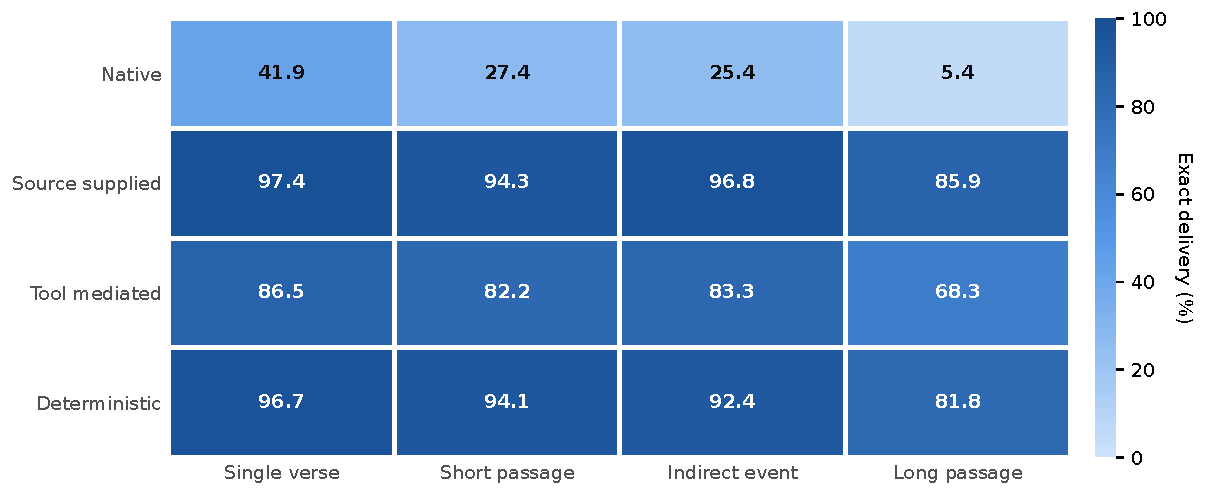
\includegraphics[width=0.88\textwidth]{fig3_passage_difficulty.pdf}
\caption{Architecture-adherent exactness by passage stratum
($N=540$ per cell). ``Indirect event'' describes target construction; both
prompt families were evaluated for every target.}
\label{fig:passage}
\end{figure}

Long passages were the most difficult stratum under every architecture
(Figure~\ref{fig:passage}). Native exactness fell to 5.37\%. Even when the
source was supplied, long-passage exactness was 85.93\%, indicating that
rendering failures were not limited to source selection. Tool and deterministic
conditions also lost accuracy through span selection before exact text could be
delivered.

\subsection{Effects varied by route but persisted across repetitions}

Every route improved substantially over its own native condition, but the
relative ordering of interventions differed (Appendix
Table~\ref{tab:model}). This
heterogeneity cautions against treating ``RAG,'' ``tool use,'' or
``deterministic rendering'' as model-independent properties.

Aggregate epoch rates were stable: 24.17--25.56\% for native, 93.47--93.75\%
for source supplied, 79.72--80.69\% for tool mediated, and 83.47--84.17\% for
deterministic rendering. Cell-level behavior was not perfectly stable. Of 720
matched cells per condition, all three epochs succeeded in 122 native, 650
source-supplied, 504 tool-mediated, and 537 deterministic cells. Repetition
therefore added information beyond a single run.

\subsection{Failure review located errors at different stages}

After primary scores were frozen, we conducted a route-blinded qualitative
review. Six failure strata were defined and five observations per stratum were
selected by a deterministic SHA-256 ordering of trial identifiers. The review
was descriptive and did not alter scores.

Native failures included near-exact surface differences, lexical drift toward
another familiar rendering, incomplete spans, blended wording, and refusals.
Source-supplied failures included both typography-only differences and
substantive alteration or omission. Tool failures separated into bypass,
tool-like text without an executable call, and authentic retrieval of the
wrong boundaries. Deterministic selection failures frequently expanded an
event to include narrative setup, narrowed a requested range to its most
salient verse, or appended an edition label that violated the strict interface.

These observations support mechanism-level interpretation, not subtype
prevalence estimates. No raw response is included in the public manuscript.

\subsection{Provider errors did not explain the main result}

Complete-case sensitivity changed native exactness from 25.00\% to 25.38\%
and tool exactness from 80.09\% to 80.13\%; the all-scheduled-observation
analysis remains primary.

The run used 1,954,958 input tokens, 3,285,730 output tokens, and 2,772,266
reasoning tokens. The execution recorded 11,483 provider API attempts,
including bounded transport retries, and 10,641 successful model responses.
Provider-attempt counts are not equivalent to semantic turns.

\section{Discussion}
\label{sec:discussion}

\subsection{Quotation reliability moved through the source-delivery chain}

The simplest reading of the primary table is that source-connected
architectures outperformed generation from memory. That is true, but
incomplete. The more useful finding is that each architecture made a different
part of the journey reliable.

Source supply made identification and retrieval unnecessary, leaving
preservation as the main risk. Tool mediation gave the model access to a source
of record, but also gave it decisions about whether to call the tool and which
span to request. Deterministic rendering made the words reliable after a
successful handoff, while leaving reference selection exposed. The failures
did not disappear as architecture changed; they migrated toward the remaining
model-owned decisions.

The study therefore does not show that deterministic rendering is universally
better than source-supplied quotation. It shows why guarantees must be assigned
to stages. A renderer can guarantee the bytes it emits without guaranteeing
that the model asked for the right source. A tool can make authoritative text
available without guaranteeing that the model will use it. And a source placed
in context can still be changed by the generative layer that presents it.

\subsection{Implications for frontier AI systems}

For frontier labs and application developers, the results suggest five design
principles.

\begin{enumerate}[leftmargin=*,topsep=4pt,itemsep=2pt]
  \item \textbf{Treat exact quotation as an intent class.} A system should
        distinguish requests for meaning from requests for exact source text.
  \item \textbf{Make the source of record explicit.} Work, edition, span,
        authorization, and retrieval provenance should be represented in the
        system state rather than inferred only from generated prose.
  \item \textbf{Separate selection from rendering.} Structured selection makes
        upstream uncertainty observable and permits a non-generative component
        to own final text.
  \item \textbf{Verify tool behavior, not tool availability.} A tool definition
        does not establish invocation, correct lookup, or faithful rendering.
  \item \textbf{Test the final user-visible buffer.} Exact source bytes can
        still be lost through truncation, wrappers, streaming errors, or later
        generative transformation.
\end{enumerate}

These principles generalize naturally to statutes, standards, policy manuals,
clinical instructions, contracts, and other materials where a source of record
exists. Generalization of the measured effect sizes, however, requires
domain-specific replication.

\subsection{Implications for Christian institutions}

The results give Christian organizations a reason to distinguish ``the model
knows this passage'' from ``the system delivered this edition faithfully.''
Native generation was especially unreliable for long passages and for the LSV
edition. A fluent response should not be assumed to preserve the requested
translation.

Three checks follow directly from the results and can be applied to a system an
institution is evaluating. Ask whether the requested edition is named and
carried through to the delivered text rather than inferred. Ask for evidence
that an authorized source was actually consulted for the requested span, since
the availability of a lookup tool did not establish its correct use here. And
test long passages and event-style requests specifically, because both degraded
under every architecture we evaluated.

These results also put a measured figure beside a widely circulated industry
estimate that models misquote Scripture between 15\% and 60\% of the time
\citep{gruenewald2026misquotes}. Native generation failed our strict endpoint
in 75.00\% of observations, which falls inside that range without replicating
it: our endpoint demands an exact match to a specified edition on a purposive
twenty-passage panel, and the circulated estimate states no protocol. The
comparison is offered as calibration, not confirmation.

At the same time, textual fidelity should not be confused with theological
fidelity. An exact verse can be detached from its literary context, used to
answer the wrong question, or interpreted contrary to a community's
confessional commitments. The present evaluation can help institutions remove
misquotation as one failure mode. It cannot decide which passage should be
used, how it should be interpreted, or what pastoral counsel should follow.
Those tasks require human judgment and, in many settings, accountable ecclesial
authority.

\subsection{What made requests harder}

Two factors changed the character of the task. First, contextual requests
required the system to infer a passage before delivering it, and the prompt
results show why that extra step deserves separate treatment. When the exact
source was already supplied, contextual wording barely changed performance.
When the system had to identify and retrieve a passage, contextual descriptions
exposed boundary and selection errors. This is not noise around the same task;
it is an additional reasoning stage.

Second, the requested edition mattered most when the model generated from
memory. Lower native exactness for LSV may reflect source availability,
memorization, translation distinctiveness, endpoint behavior, or other
factors. The study
documents the interaction without treating ``familiarity'' as a measured
training-data variable.

\section{Open Evaluation and Reproducibility}
\label{sec:open-release}

The public repository is available at
\url{https://github.com/FideAI/scripture-quotation-fidelity}. It releases:

\begin{itemize}[leftmargin=*,topsep=4pt,itemsep=2pt]
  \item this paper and citation metadata;
  \item the authoritative-quotation methodology and scoring specification;
  \item scenario and reference schemas;
  \item the exact executed prompts, functional tool schema, and release-safe
        target registry;
  \item the source-edition record, with per-target normalized-text digests for
        every edition in the locked registry;
  \item a deidentified 8,640-row derived-score dataset that excludes generated
        prose and source text;
  \item reviewed aggregate and target-level tables and a result card;
  \item the prospective-lock receipt and deviation summary;
  \item standalone code for the target-level, target-cluster bootstrap, and
        post-hoc cluster-robust analyses;
  \item claims, responsible-use, and release policies; and
  \item documentation mapping the public methodology to a private execution
        engine.
\end{itemize}

The public repository excludes private runner code, credentials, provider
response identifiers, raw model outputs, held-out prompts, partner-private
traces, and restricted source text. This is a deliberate reproducibility
boundary. The released derived scores and analysis code reproduce the
quantitative claims without network access. An exact endpoint rerun remains
subject to model and routing drift and requires an independent execution
implementation plus appropriately authorized sources.

The shared condition implementation was executed from a pinned revision of The
Apologist Project's \texttt{llm-scripture-fidelity} repository. Fide AI
controlled the crossed design, credentials, execution, scoring review, claims
boundary, and result custody. The collaboration does not constitute product
certification or commercial endorsement. The partner may publish a separate
companion explanation of its implementation.

\section{Responsible Use and Limitations}
\label{sec:limitations}

This work is a measurement study. It is not legal advice, copyright clearance,
theological certification, pastoral-safety approval, product endorsement, or
deployment authorization.

Rights status is an architectural input. BSB and WEBU were evaluated as
public-domain sources; LSV was used under its stated open license, with no LSV
passage text included in the public result package. Restricted translations
require separate source and source-to-model authorization. Technical ability
to reproduce text does not itself establish a right to distribute it.

For Christian readers, ``fidelity'' has a deliberately narrow meaning here:
fidelity to the requested English source text and span. Christian traditions
also use the term for faithfulness to Scripture's meaning, canonical context,
doctrine, and lived obedience. Nothing in the experiment reduces those
questions to string matching.

\subsection{Limitations of the current study}

\paragraph{Purposive target panel.}
The twenty passages were selected to expose distinct technical behaviors.
They do not estimate the prevalence of quotation failure across the Bible, all
Christian use cases, or ordinary user traffic.

\paragraph{English and Scripture only.}
The experiment used three English editions and one sacred-text domain.
Reference conventions, translation ecosystems, source authority, and language
technology differ elsewhere. Cross-lingual and cross-domain claims require new
studies.

\paragraph{Edition versioning.}
Ground truth was a fixed stored copy of each edition, verified stable by
repeat-fetch digests across the run and disclosed in the released
source-edition record. Open English editions are nonetheless revised over
time, so an exact replication requires the same edition version, not merely
the same edition name; the released per-target digests let a replicator
confirm that condition before running anything. The digests establish that our
ground truth was internally stable and externally checkable, not that the
upstream provider's text is itself authoritative for a given publisher.

\paragraph{Open editions only.}
The primary experiment does not measure restricted translations. It therefore
cannot establish how licensing, provider quotation policies, or source-transfer
permissions affect the four architectures.

\paragraph{Model and route drift.}
Results apply to six named routes on July 26--27, 2026. Hosted models, routing,
guardrails, and provider defaults can change. Three epochs measure short-run
variability, not longitudinal stability.

\paragraph{Provider-default sampling.}
Temperature and other generation controls were omitted and left at provider
defaults. This improves ecological comparability to the evaluated access path
but limits causal interpretation of sampling parameters.

\paragraph{Strict interface contract.}
The deterministic primary result includes failures caused by a deliberately
strict reference grammar. Tolerant analysis shows that many syntax-tagged
outputs contained the intended reference. A production system could adopt a
more permissive parser, but changing the parser after observing results would
invalidate the locked primary comparison.

\paragraph{Automated exactness.}
Exact matching is appropriate for the declared endpoint, but failure tags and
normalized views depend on implementation choices. A post-run route-blinded
review checked mechanisms in a small diagnostic sample; it was not a second
population annotation study.

\paragraph{Dependence and fixed-panel inference.}
Target-cluster bootstrap intervals describe variation within this target
panel, while model routes and editions remain fixed. Target-level distributions
and a post-hoc target-cluster-robust fixed-panel sensitivity analysis make this
dependence visible, but neither supports population inference to all Scripture
requests, models, or editions. With only twenty target clusters, uncertainty
estimates remain coarse; a larger probability-oriented target sample would be
needed for population claims.

\paragraph{Contextual-description review.}
The six revised contextual descriptions received a structurally blinded
technical reapproval, but the reviewer was an AI system and the same reviewing
identity that authored the initial critique. This supports an internal
construct check, not independent credentialed scholarly validation. The
contextual-prompt results should be read with that limitation attached: a low
reference-identification rate could reflect system behavior or description
quality, and the present evidence does not fully separate them. Materials for
an independent scholarly review of all twenty descriptions---protocol, blinded
packet, and pre-committed scoring rules---are released with this package so
that check can be carried out and reported by us or by others. Primary scores
are frozen, so such a review can qualify how the contextual-prompt findings are
interpreted but cannot alter any reported quantity.

\paragraph{No contextual or theological endpoint.}
Contextual descriptions test technical reference identification. The study
does not determine whether the expected passage is the best theological,
exegetical, or pastoral response to a real person's situation.

\section{Conclusion}
\label{sec:conclusion}

AI systems should not always generate. In this study, native parametric
quotation delivered the requested edition exactly in 25.00\% of observations.
Supplying authoritative text, connecting a source tool, or delegating final
rendering to a deterministic layer all produced large improvements, but none
eliminated failure. Each architecture moved failure to the decision it still
left to the model.

The practical lesson is not that one method wins every comparison. It is that
authoritative quotation should be designed and evaluated as a sequence of
observable responsibilities. Models may identify what a user means. Source
interfaces may retrieve what is authorized. Deterministic components may
render what must not change. Final-output checks must establish what the user
actually received.

Return to the opening request about Jesus and the serpent in the wilderness.
The system should be able to show whether the model identified the intended
passage, whether an authorized source supplied the requested edition, and
whether the final words survived intact. If the answer is wrong, the same
chain should reveal whether the error was selection, access, or rendering.

Scripture makes these distinctions visible, but the underlying problem belongs
to any AI system that handles authoritative text. When wording is material, the
system should be able to say when the model is speaking and when the source of
record is speaking.

\section*{Data and Code Availability}

The public repository,
\url{https://github.com/FideAI/scripture-quotation-fidelity}, releases the full
deidentified derived-score dataset, target registry, executed prompt templates,
functional tool schema, source-edition record with per-target text digests,
release-safe prospective-lock and deviation records, and standalone analysis
code. It excludes generated prose, authoritative passage text, provider
response identifiers, raw tool traces, credentials, restricted-source
payloads, and private execution-engine code. The released package reproduces
the quantitative tables and contrasts without model endpoint access.

\section*{Author Contributions}

Alex Chao: conceptualization, methodology, study design, software integration,
validation, formal analysis, investigation, data curation, visualization,
writing, supervision, and project administration.

\section*{Competing Interests and Collaboration}

The Apologist Project collaborated on and maintains the shared condition
implementation used for local execution. Fide AI controlled the methodology,
prospective lock, credentials, confirmatory execution, analysis, evidence
custody, release decision, and claims boundary. The Apologist Project develops
commercial technology related to Scripture delivery, creating an organizational
interest relevant to the study topic. The study did not evaluate or certify a
deployed commercial product.

\section*{Use of AI Systems}

AI systems assisted with code generation, manuscript drafting, citation
cross-checking, and internal contextual-description review. Quantitative
outcomes were produced by the declared automated scoring pipeline. The AI
review is disclosed as an internal construct check and is not represented as
independent credentialed scholarly validation.

\appendix

\section{Target References}
\label{app:targets}

The twenty target references were: John 3:16; Genesis 1:1; Romans 8:28;
Hebrews 11:1; John 14:6; Psalm 23:1--3; Proverbs 3:5--6; Ephesians 2:8--9;
Philippians 4:6--7; Deuteronomy 6:4--5; Matthew 5:3--10;
1 Corinthians 13:4--7; Isaiah 53:4--6; Revelation 21:1--4;
Matthew 22:37--40; Numbers 21:8--9; John 3:14--15; Luke 2:10--12;
Micah 6:8; and James 1:5.

The public repository includes all twenty release-safe target records and the
exact contextual descriptions. Generated outputs and authoritative source text
remain governed by the release policy.

\section{Execution Routes and Prospective Lock}
\label{app:routes}

The executed OpenRouter model identifiers and pinned upstreams were:
\texttt{openai/gpt-5.6-sol} via OpenAI;
\texttt{anthropic/claude-sonnet-5} via Anthropic;
\texttt{google/gemini-3.5-flash} via Google AI Studio;
\texttt{deepseek/deepseek-v4-pro} via Together;
\texttt{moonshotai/kimi-k3} via Moonshot; and
\texttt{z-ai/glm-5.2} via Together. Fallbacks were disabled, required parameter
support was enabled, and data-collecting routes were denied.

The internal prospective lock was recorded at
\texttt{2026-07-26T22:28:40Z}. Confirmatory execution began at
\texttt{2026-07-26T23:11:30Z}. The lock identified the target pack, execution
matrix, contextual annotations, source panel and registry, scoring rubric,
manifest, and deviation log by SHA-256 digest. These records are intended for
the archival replication package.

\section{Route-by-Condition Results}
\label{app:route-results}

\begin{table}[h]
\centering
\small
\begin{tabular}{lrrrr}
\toprule
Evaluated route & Native & Source supplied & Tool & Deterministic \\
\midrule
Claude Sonnet 5 & 12.78\% & 82.22\% & 78.06\% & 75.56\% \\
DeepSeek V4 Pro & 32.22\% & 96.11\% & 83.61\% & 89.17\% \\
Gemini 3.5 Flash & 16.11\% & 98.06\% & 86.94\% & 91.94\% \\
GLM-5.2 & 20.00\% & 93.61\% & 75.56\% & 85.83\% \\
GPT-5.6 Sol & 35.28\% & 97.22\% & 92.50\% & 71.39\% \\
Kimi K3 & 33.61\% & 94.44\% & 63.89\% & 89.72\% \\
\bottomrule
\end{tabular}
\caption{Descriptive route-by-condition architecture-adherent exactness
($N=360$ per cell). Rows are ordered alphabetically, not by performance; this
is not a model leaderboard.}
\label{tab:model}
\end{table}

\section{Failure Tags}
\label{app:failure-tags}

Observed structured tags included 345 wrong or unparseable deterministic
reference selections, 234 tool calls that did not retrieve the requested span,
161 invalid deterministic reference payloads or placeholder failures, 161
selected-reference lookup failures, and 107 tool-bypass observations. Tags
can co-occur and must not be summed as unique failed observations. Native and
source-supplied text mismatches are represented primarily through exact,
normalized, coverage, and answer-presence metrics rather than these
architecture-specific tags.

\section{Claims Boundary}
\label{app:claims}

Results apply only to the named routes, dates, twenty-target panel, two prompt
families, three open English editions, four architecture conditions, and
declared scoring protocol. The study does not establish:

\begin{itemize}[leftmargin=*,topsep=4pt,itemsep=2pt]
  \item a general ranking of models or vendors;
  \item theological truth or contextual appropriateness;
  \item pastoral safety or institutional deployment readiness;
  \item training-data membership or memorization causation;
  \item universal legal or licensing compliance;
  \item performance on restricted translations; or
  \item superiority of a commercial product.
\end{itemize}

\bibliographystyle{acl_natbib}
\bibliography{references}

\end{document}
